\chapter{Diseño e implementación} % Main chapter title

En este capítulo se van a describir las soluciones planteadas al problema resuelto en este trabajo.

%----------------------------------------------------------------------------------------
%	SECTION 1
%----------------------------------------------------------------------------------------
\section{Arquitectura del sistema}

En la figura \ref{fig:arqSistema} se puede observar un esquema simple del sistema, donde se tiene:

\begin{itemize}
	\item Nodos sensores.
	\item Nodo Central.
	\item Aplicacion web progresiva.
	\item Broker.
	\item Servidor IoT.
\end{itemize}

\begin{figure}[H]
\centering 
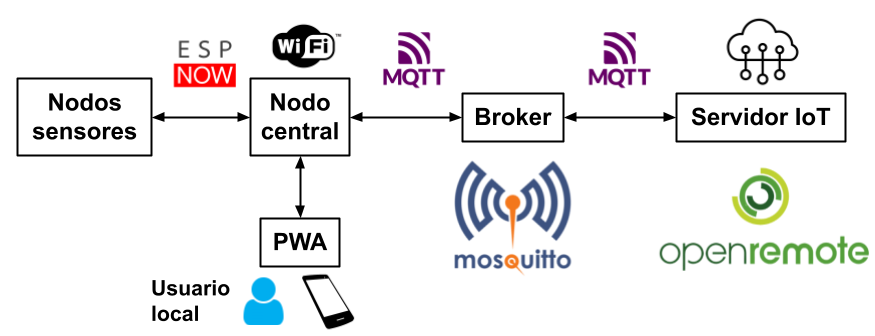
\includegraphics[width=1\textwidth]{./Figures/arq_sistema.png}
\caption{Esquema del sistema.}
\label{fig:arqSistema}
\end{figure}

En esta sección se describen los principales módulos que conforman el sistema, detallando su función y cómo interactúan entre sí.

\subsection{Nodos sensores} 

Están conformados por un módulo ESP32-C3 y un sensor. Esta es la capa de percepción, ya que los nodos son responsables de captar la información del entorno. Los datos recopilados son enviados al nodo central (gateway) a través del protocolo de comunicación ESP-NOW. En este contexto, también se incluye un módulo específico para gestionar los relés, cuyo estado puede ser consultado y modificado, por lo que se establece una \textit{comunicación bidireccional} con el \textit{gateway}. Sin embargo, en el caso de los sensores, la \textit{comunicación es unidireccional}, ya que solo envían datos.

\subsection{Nodo central}

Como se mencionó, este nodo se comunica con los sensores a través de ESP-NOW. Actúa como la capa de transporte, encargándose de transferir los datos capturados por la capa de percepción. Además, el \textit{gateway} integra una interfaz web embebida para visualizar los datos de los sensores y el estado de los relés. Esta interfaz está implementada utilizando un socket y, en caso de ausencia de conexión a internet, genera un “Access Point” (AP) local al cual el usuario puede conectarse para monitorear el estado del invernadero. El nodo central se conecta a internet mediante Wi-Fi para enviar los datos a un \textit{broker} MQTT (Mosquitto), empleando certificados TLS para asegurar la transmisión.

\subsection{Servidor IoT}

Este componente corresponde a la capa de procesamiento, donde se almacenan, analizan y gestionan los datos enviados desde el nodo central. Para esta función, se utilizará \textit{OpenRemote} como plataforma de servidor IoT, la cual facilita la integración de dispositivos y la gestión de datos. El servidor se conecta al \textit{broker} MQTT para recibir la información de los sensores y los relés.
Además de almacenar y visualizar los datos en tiempo real, el servidor permite generar informes, configurar alertas y ejecutar acciones automatizadas basadas en reglas predefinidas, como la activación de relés o notificaciones ante condiciones anómalas.



%----------------------------------------------------------------------------------------
\section{Desarrollo del firmware}

El \textit{firmware} del trabajo fue desarrollado utilizando el lenguaje de programación \textit{Python}, específicamente bajo el \textit{framework MicroPython}. Para su implementación, se empleó el entorno de desarrollo Visual Studio Code, que facilitó la edición y depuración del código.

En esta sección se presentan los diagramas de flujo que describen los procesos clave de los nodos sensores, el módulo de relés y el nodo central. Estos diagramas ilustran la lógica implementada en el \textit{firmware} y cómo se gestiona la comunicación eficiente entre sensores, actuadores, la interfaz web y el servidor IoT.

\subsection{Nodos sensores y módulo relés}

\subsubsection{Nodos sensores}

En la figura \ref{fig:flujoSensor} se presenta el diagrama de flujo de los nodos sensores. 

Cada sensor tendrá un script personalizado, ya que son diferentes entre sí, lo que implica que la forma de obtener las lecturas de los datos variará en cada caso. Sin embargo, el procedimiento para enviar los datos será el mismo para todos.

Primero, se inicializa y configura ESP-NOW para enviar mensajes en modo \textit{broadcast} (difusión) a todos los dispositivos cercanos, sin la necesidad de conocer sus direcciones MAC individuales
A continuación, el nodo busca el canal en el que se encuentra el \textit{gateway}. Una vez encontrado, se envía un mensaje de verificación para confirmar que el canal es el correcto. Si no se recibe respuesta, el nodo se reinicia, comenzando el proceso nuevamente.

Cuando el canal es verificado, se toma la lectura de los datos del sensor y se envía esta información al \textit{gateway} vía ESP-NOW, de forma encriptada, utilizando una librería específica de \textit{MicroPython} llamada \textit{cryptolib} \citep{docsmpy}.

Una vez que la información ha sido enviada, el dispositivo entra en \textit{modo DeepSleep} (sueño profundo) durante un tiempo determinado, con el fin de ahorrar energía. Al despertar, el módulo se reinicia como si hubiese sido encendido nuevamente.

\begin{figure}[H]
\centering 
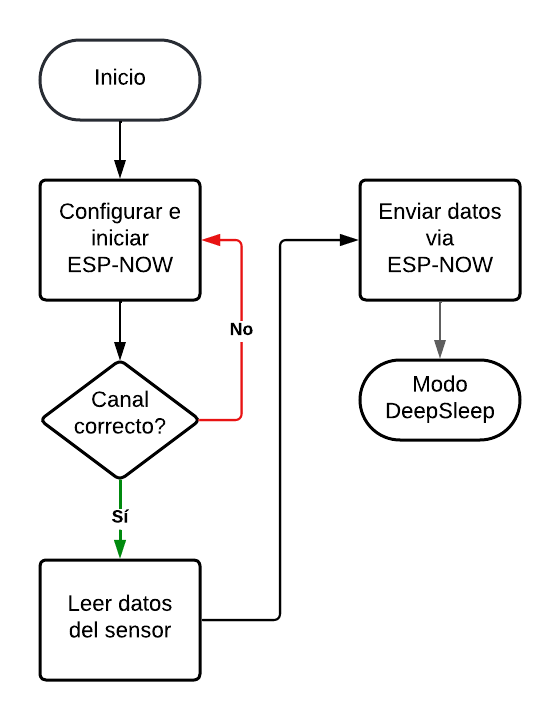
\includegraphics[width=0.5\textwidth]{./Figures/flujo_nodo_sensor.png}
\caption{Diagrama de flujo de los nodos sensores.}
\label{fig:flujoSensor}
\end{figure}

\subsubsection{Módulo relés}

El nodo encargado de los relés sigue un funcionamiento similar al de los nodos sensores en cuanto a la configuración inicial de ESP-NOW, por lo que no es necesario volver a detallar ese proceso. La principal diferencia radica en que, en lugar de tomar lecturas de un sensor, este nodo inicializa los relés y envía el estado en el que se encuentran al \textit{gateway}.

Una vez enviados los estados, el nodo queda a la espera de recibir instrucciones para modificar alguno de los relés. Si se recibe una solicitud para cambiar el estado de uno o más relés, el nodo ejecuta el cambio y, a continuación, envía nuevamente la información actualizada al \textit{gateway}.
Al igual que en los nodos sensores, la información se envía de forma encriptada para garantizar la seguridad de los datos transmitidos. De la misma manera, cualquier información que llega al nodo, como instrucciones para cambiar el estado de los relés, es desencriptada antes de ser procesada.

Este nodo no entra en \textit{modo DeepSleep}, ya que es necesario garantizar que los relés respondan de manera inmediata a cualquier instrucción de control que pueda recibirse.

En la figura \ref{fig:flujoRele} se puede observar el diagrama de flujo del módulo relés. 

\begin{figure}[H]
\centering 
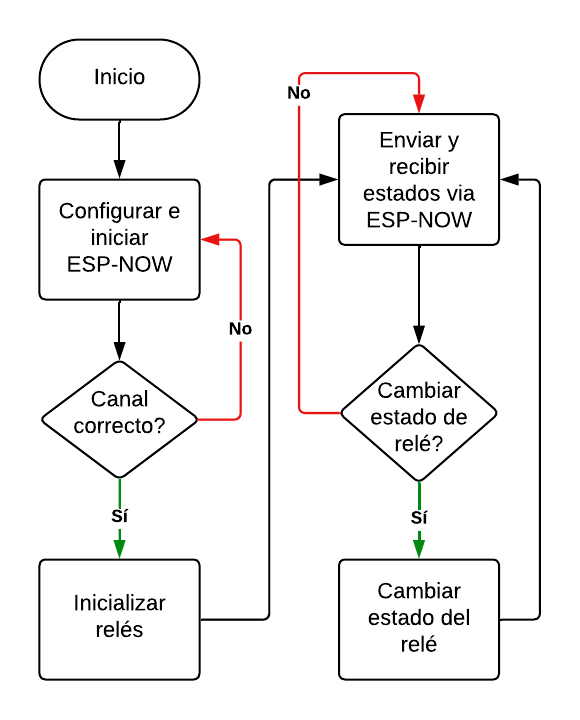
\includegraphics[width=0.5\textwidth]{./Figures/flujo_rele.png}
\caption{Diagrama de flujo del módulo relés.}
\label{fig:flujoRele}
\end{figure}

\subsection{Nodo Central}

El \textit{gateway} puede iniciar en dos modos diferentes: \textit{Modo Cliente} (CL) o \textit{Modo Access Point} (AP), dependiendo de la configuración cargada en el dispositivo. Una vez determinado el modo de operación, se configura e inicia la comunicación ESP-NOW en \textit{modo de difusión}.

\begin{itemize}
	\item Modo AP: en este caso, el \textit{gateway} actúa como un punto de acceso local, lo que significa que no está conectado a internet. Se inicia el servidor HTTP para proporcionar una interfaz web accesible a través de una red local, permitiendo al usuario monitorear y gestionar el sistema directamente sin necesidad de conexión externa.
	\item Modo CL: al iniciar en este modo significa que está conectado a internet a través de una red Wi-Fi. Se establece una conexión segura con un \textit{broker} MQTT. Para ello, se utilizan un nombre de usuario, una contraseña y certificados TLS para asegurar la comunicación. Además, el gateway se suscribe a un tópico específico del \textit{broker} MQTT, lo que le permite recibir mensajes relacionados con los sensores. Por último se inicia el servidor HTTP, lo que permite el acceso a la interfaz web embebida para monitorear y gestionar el sistema desde cualquier lugar con acceso a internet.
\end{itemize}

En la figura \ref{fig:flujoCentral} se puede observar el diagrama de flujo general del nodo central. 

\begin{figure}[H]
\centering 
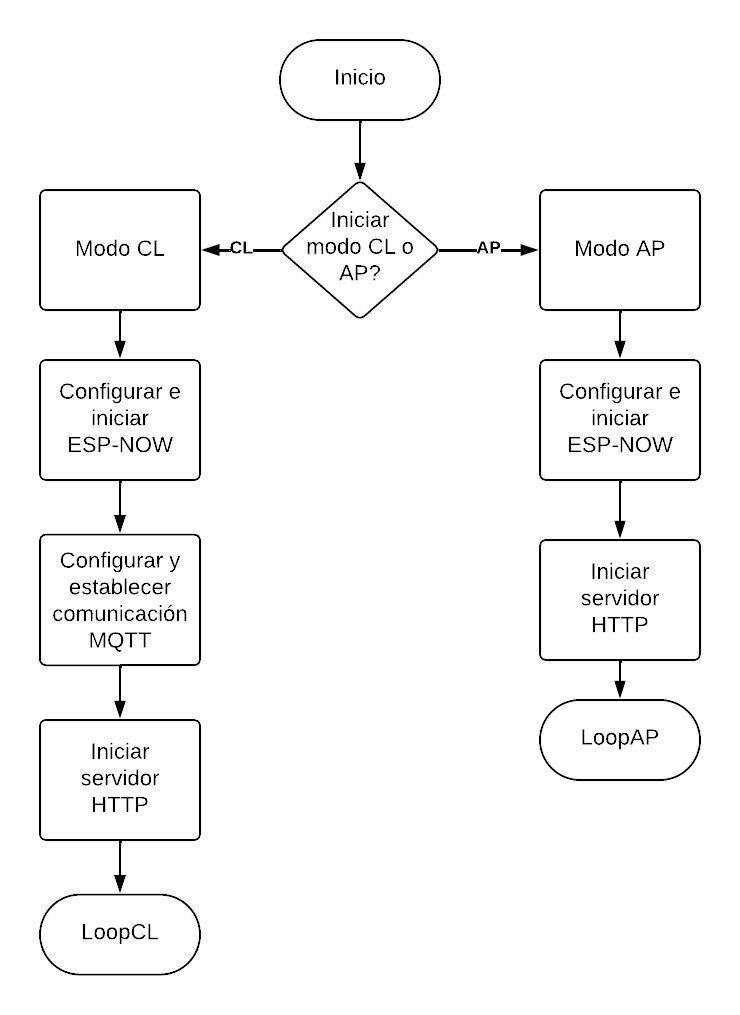
\includegraphics[width=0.7\textwidth]{./Figures/flujo_central.png}
\caption{Diagrama de flujo del nodo central.}
\label{fig:flujoCentral}
\end{figure}

\subsubsection{Loop AP}

En la figura \ref{fig:flujoAP} se puede observar el diagrama de flujo del loopAP. 

Una vez que el \textit{gateway} se ha iniciado en Modo AP y se ha configurado correctamente la comunicación ESP-NOW, entra en un bucle continuo de monitoreo y control, conocido como LoopAP. En este modo el \textit{gateway} realiza las siguientes acciones:

\begin{itemize}
	\item Monitoreo de nodos: el \textit{gateway} espera recibir datos de los nodos sensores y del módulo de relés a través de ESP-NOW. Al recibir información, ya sea de sensores o del estado de los relés, estos datos se envían y muestran en la PWA en tiempo real.
	\item Verificación de cambios en la PWA: si no se recibe información desde los nodos, el \textit{gateway} revisa si hubo un cambio en el estado de los relés en la PWA. Si detecta un cambio, envía la actualización al nodo correspondiente mediante ESP-NOW.
	\item Reinicio del ciclo: luego de procesar cualquier evento, el \textit{gateway} regresa al inicio del ciclo, quedando en espera de nuevos datos o cambios.
\end{itemize}


\begin{figure}[H]
\centering 
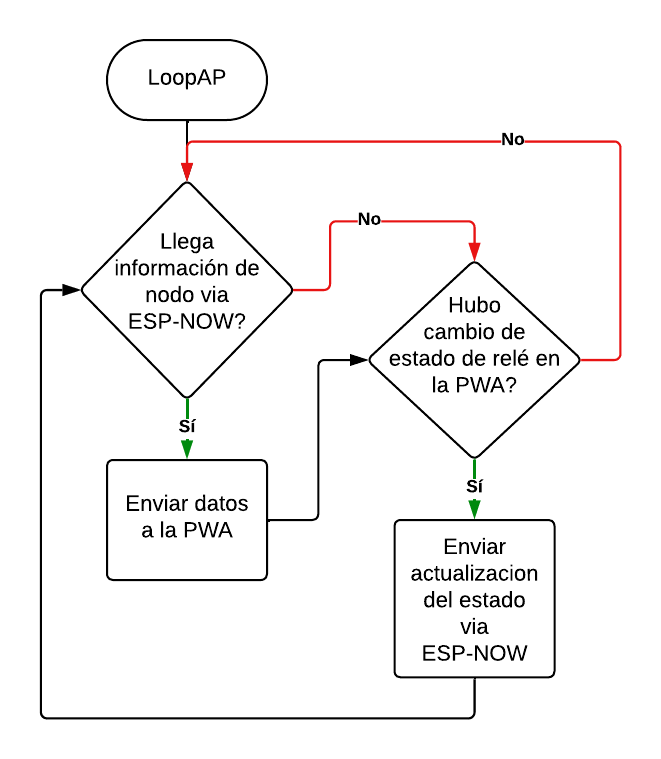
\includegraphics[width=0.5\textwidth]{./Figures/flujo_ap.png}
\caption{Diagrama de flujo del loop AP.}
\label{fig:flujoAP}
\end{figure}

\subsubsection{Loop CL}

En este modo, los datos de los sensores no solo se muestran localmente en la PWA, sino que también se publican en el \textit{broker} MQTT, lo que permite que sean almacenados y procesados remotamente. Esto garantiza una mayor capacidad de monitoreo y análisis.
Otra diferencia importante es la sincronización con el servidor IoT. Mientras que en el LoopAP los cambios en el estado de los relés solo se controlan desde la PWA, en el LoopCL también se monitorea si el estado de los relés ha sido modificado desde el servidor IoT. Esto posibilita la gestión remota de los dispositivos, permitiendo que el usuario controle y supervise el invernadero desde cualquier lugar con acceso a internet, una funcionalidad que no está disponible en el modo AP.

En la figura \ref{fig:flujoAP} se presenta el diagrama de flujo del loopCL. 

\begin{figure}[H]
\centering 
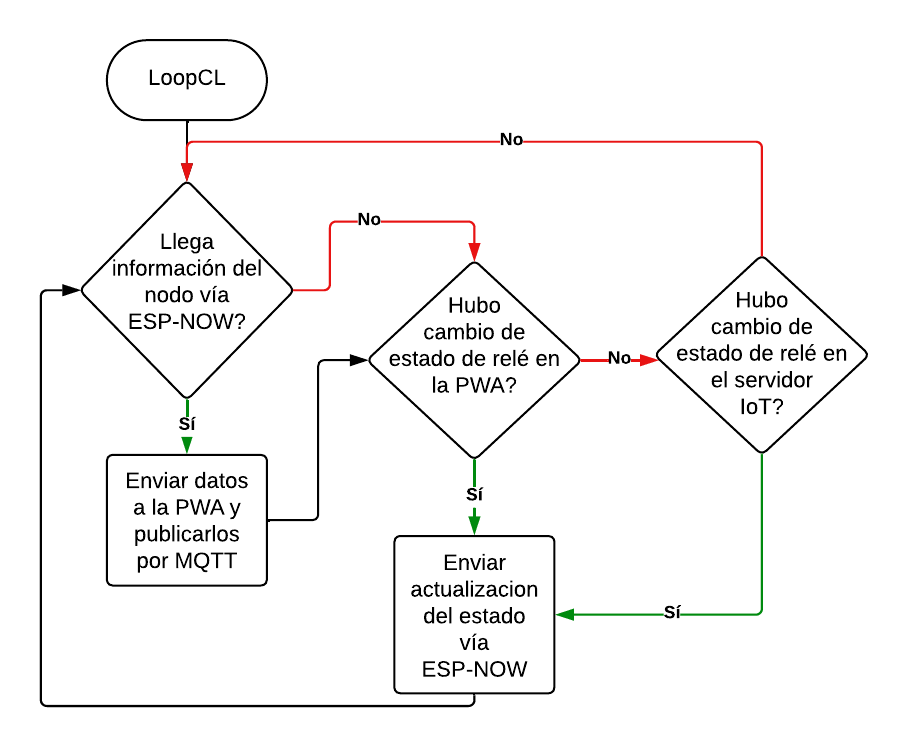
\includegraphics[width=0.6\textwidth]{./Figures/flujo_cl.png}
\caption{Diagrama de flujo del loop CL.}
\label{fig:flujoCL}
\end{figure}

%----------------------------------------------------------------------------------------
\section{Desarrollo de la aplicacion web progresiva}

%----------------------------------------------------------------------------------------
\section{Implementación del servidor IoT}

%----------------------------------------------------------------------------------------
\section{Despliegue del sistema}



